\subsection{ Hidden Markov Model }
For this Hidden Markov Model, we use all the features we described in the previous section. Here, we try to label each word in a sentence as \{YES, NO\}. This method is different from the earlier method in a way that we consider state transition probabilities are considered. It is likely to perform better.
 

\noindent \textbf{Training}
\begin{enumerate}
\item {50 news articles, its title and meta data extracted from Yahoo! News are used as training data.}
\item {In the metadata text all stopwords are removed. The remaining words in metadata are considered as keywords.}
\item { Each word in news article is looked up in metadata text, if found it is tagged as `YES' else tagged as `NO'. }
\end{enumerate}

For the new document the each word is tagged `YES' or `NO'. The words which are tagged as `YES' considered to be keywords.

The Best key sequence is 
\begin{equation}
KeySeq^{*} = argmax_{KeySeq} P(KeySeq / Word, PosTag, IDFTF, titleScore) 
\end{equation}

\begin{figure}[H]
\begin{center}
\fbox{\scalebox{0.7}{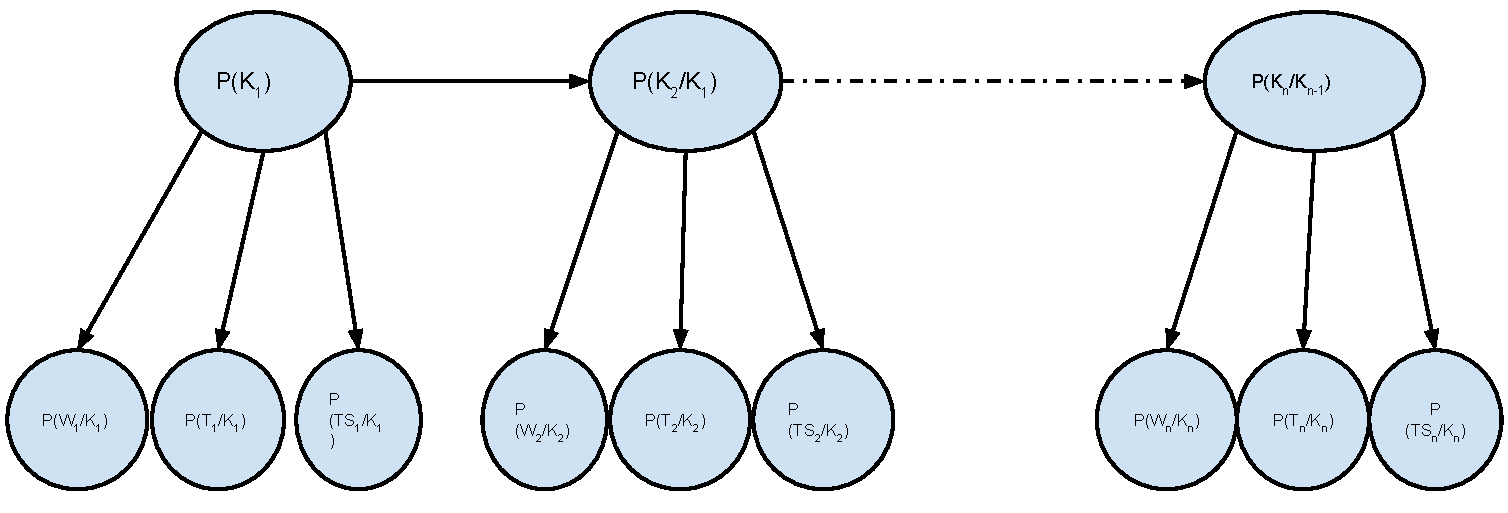
\includegraphics{hmm.pdf}}}
\end{center}
\caption{Hidden Markov Model}
\end{figure}



\noindent $
P(KeySeq / Word, PosTag, IDFTF, titleScore) 
$
\begin{align}
=& P(KeySeq) * P(Word, PosTag, IDFTF, titleScore / KeySeq)  \\
\intertext{Using chain rule,}
=& P(KeySeq) * P(Word/KeySeq) * P(PosTag/KeySeq,Word) \nonumber \\
 & *  P(IDFTF/KeySeq, Word, PosTag)  * P(titleScore/KeySeq,KeySeq, Word, PosTag, IDFTF) \\
\intertext{Independence assumptions,}
=& P(KeySeq) * P(Word/KeySeq) * P(PosTag/KeySeq) P(IDFTF/KeySeq) * P(titleScore/KeySeq) 
\intertext{Using markov assumption,}
=& P(Key_{1}) * P(Key_2/Key_1) *.. * P(Key_n/key_{n-1}) *  \nonumber \\ 
 & P(Word_1/Key_1) * P(Word_2/Key_2) *..* P(Word_n/Key_n) * \nonumber \\
 & P(PosTag_1/Key_1) * P(PosTag_2/Key_2) *..* P(PosTag_n/Key_n) * \nonumber \\
  & P(IDFTF_1/Key_1) * P(IDFTF_2/Key_2) *..* P(IDFTF_n/Key_n) * \nonumber \\
 & P(titleScore_1/Key_1) * P(titleScore_2/Key_2) *..* P(titleScore_n/Key_n)  
\end{align}

%\textbf{Results : } \todosmall{TODO}
